\chapter{Technologie cible et outils}\label{chap:met}
Le premier objectif proposé a été d'étudier le framework \kwplay et de s'assurer de la compatibilité de sa philosophie avec un projet de génération de code. Dans la section \ref{sec:pla} de ce chapitre, nous détaillerons les qualités de ce framework qui ont motivées la sélection de \kwplay pour ce projet. Dans un second temps (\cf{} section \ref{sec:pro}, nous aborderons le prototype que nous avons élaboré avec \kwplay. 


\section{Le Framework Play}\label{sec:pla}

\kwplay{} est un CMS (Content Management System) web basé sur les langages Java et Scala permettant de la création d'applications web. De plus en plus de développeurs choisissent cet outil, qui est relativement récent, et qui présente de nombreux avantages. L'aspect \guim{prêt à l'emploi} (\textit{Plug'n Play}) permis par ses fonctionnalités par défaut le rendent efficace et rapide à mettre en place et à configurer. Le développement également est facilité, d'une part par par des mécanismes de compilation à la volée (\textit{shadow-build}) lors du chargement des pages, mais aussi par la mise à disposition de systèmes tests intégrées (JUnit, Selenium). Sa gestion des requêtes Web peut être bloquante ou non-bloquante (synchronisme). La génération des pages Web renvoyées peut être dynamisée grâce à un mécanismes de templating basé sur Scala. Enfin son architecture modulaire, composée de plugins et du \textit{design pattern} MVC (Modèle-Vue-Contrôleur), permettent une répartition claire du code source ce qui est propice à la démarche MDA. %TODO (MDA : terme à définir en début de rapport).

\begin{figure}[htb]
  \centering
  
\includegraphics[scale=.3]{img/logoPlay.eps}
  \caption{Framework Play!}
  \label{fig:play}
\end{figure}


Le Framwork \kwplay{} propose de diviser l'implémentation d'un site web en trois composantes principales :

\subsection{Les pages web}
% Parler vite fait du templatage scala
Pour la gestion de ses pages web, \kwplay{} propose une approche basée sur les templates. Les pages peuvent donc être écrites avec du HTML classique, et être enrichies avec du code \kwscala{} pour générer du contenu dynamiquement. Ainsi, il est possible d'insérer des clauses conditionnelles (if/else) ou des boucles (for/while) à l'intérieur du code HTML. Afin de conserver une architecture cohérente, il est possible de passer un certain nombre d'arguments/objets en paramètre de ces templates, afin que les pages puissent en afficher le contenu de manière formatée.

\subsection{Les Données}
% Parler de l'ORM ebean
La gestion des données dans \kwplay{} est laissée au choix de l'utilisateur - le développeur. Cependant, \kwplay{} embarque nativement l'ORM \kwebean{}. Le principe d'un ORM (Object-Relational Mapping) est de fournir une couche d'abstraction dessus d'une Base de Données relationnelle. Cette couche d'abstraction doit être suffisante pour que les différents éléments de la base soient manipulables directement en tant qu'Objets. Cela permet aux développeurs de s'affranchir des contraintes techniques que peuvent présenter les Bases de Données relationnelles.\\
Dans \kwplay{}, avec \kwebean{}, une classe Java pourra être gérée comme étant une entité/table, et ses attributs et références seront traitées comme des colonnes de cette table.
(!!! Hésitez pas à annoter les points où c'est pas clair, car c'est un peu capilotracté des fois !!!)

\subsection{Les Contrôleurs et les Routes}
%Expliquer leur role
Dans \kwplay{} le/les contrôleur(s) joue(nt) un rôle central au sein l'application. Ce sont les contrôleurs qui se chargent de récupérer les requêtes des visiteurs (de type HTTP), d'effectuer les traitements (ajout d'un cookie, traitement dans la Base de Données, ...), et d'effectuer le rendu des pages web retournées au visiteur.\\
Dans le monde du Web, les requêtes se présentent la plupart du temps sous forme d'adresse dite URL (Uniform Resource Locator) appelée par le visiteur. Comme beaucoup d'autres CMS, \kwplay{} propose un fichier de Routes dans sa configuration. Le rôle d'un fichier de Routes est de convertir/résoudre les adresses/URL afin de les faire correspondre à une méthode du Contrôleur de l'application.\\\\
Ainsi, lorsqu'une requête arrive à l'application, \kwplay{} regarde d'abord dans son fichier de Routes, puis appelle la méthode correspondante, qui retournera une réponse/page vers l'émetteur de la requête.

\begin{figure}[htb]
  \centering
  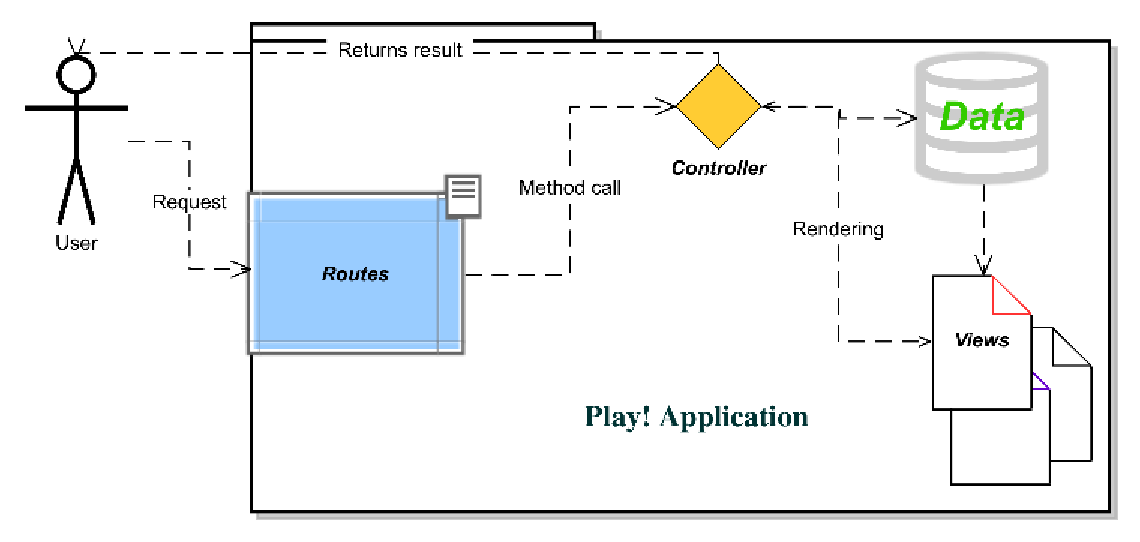
\includegraphics[scale=.8]{img/play_scheme.eps}
  \caption{Fonctionnement de Play!}
  \label{fig:play_sch}
\end{figure}

\section{Conception d’une maquette d’exemple}\label{sec:pro}

Nous nous sommes proposés de bâtir un mini-site Web basé sur \kwplay{}. L'ojectif est double :
\begin{itemize}
\item Nous familiariser avec le framework \kwplay{} et comprendre son fonctionnement.
\item Obtenir une maquette qui sera utilisée comme objectif de code à générer.
\end{itemize}

Le prototype que nous avons proposé est une implémentation simpliée d'un site marchand. Ce type de site web est en effet très courant, et il implique différents aspects et fonctionnalités : Stockage persistant de données (produits vendus), utilisation de formulaires (inscription des clients), utilisation de sessions (authentification des clients sur le site, et achats).

\begin{figure}[htb]
  \centering
  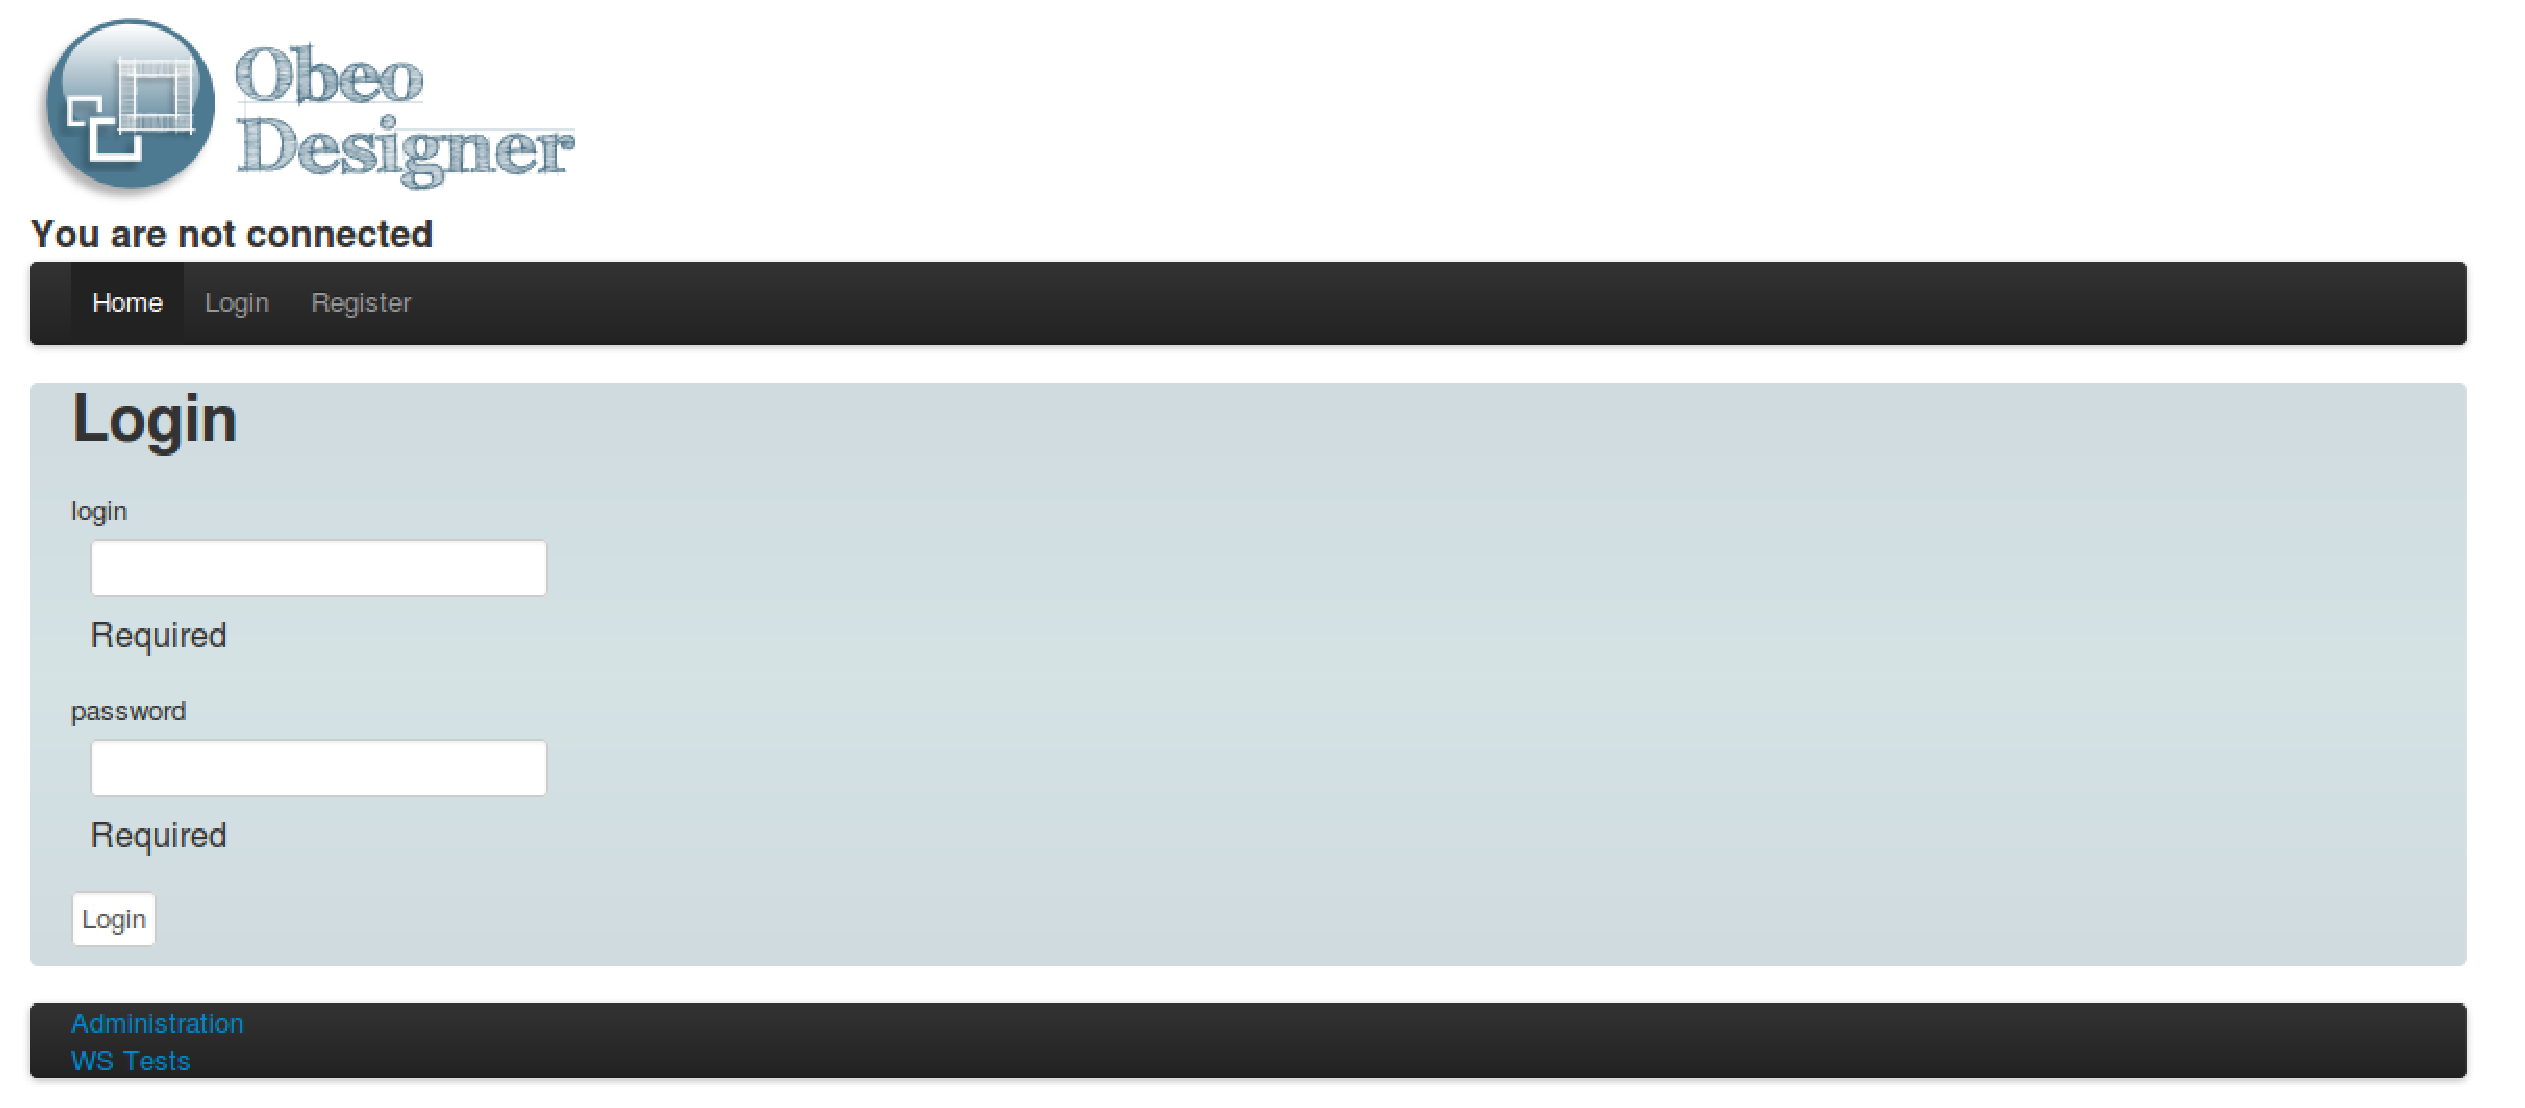
\includegraphics[scale=.2]{img/proto.eps}
  \caption{Prototype Play\_Shop}
  \label{fig:pro}
\end{figure}



%% \begin{figure}[htb]
%%   \centering
%%   \includegraphics[scale=.3]{img/Cin.eps}
%%   \caption{Méta model SOA}
%%   \label{fig:soa}
%% \end{figure}


%%  LocalWords:  framework play Scala web Plug'n shadow-build JUnit
%%  LocalWords:  Selenium non-bloquantes plugins MVC MDA woua nuull
%%  LocalWords:  refractoring implémentation Shop models Model Entity
%%  LocalWords:  méta-modèle model SOA blah bklah fdslmk
